\section{Testing and validation of bound propagation}

In this section, the results of tests on the runtime and memory usage of the new PyNeVer algorithm are presented compared to the previous version. Additionally, the results are also compared to the winners of the 2022 VNNComp (Verification of Neural Networks Competition).
A separate section is dedicated to validation tests to verify the correct functioning of the bound propagation. These tests will be performed on various networks and different properties to ensure the robustness and accuracy of the algorithm.
All these tests are conducted on different networks and various properties to cover a wide range of scenarios and validate the effectiveness of the bound propagation algorithm.
By including a section on validation tests, it ensures that the bound propagation algorithm implemented in PyNeVer produces accurate and reliable results. The tests may include specific test cases with known expected results as well as general test cases to verify and validate desired properties.
Overall, the inclusion of tests on diverse networks and properties, along with comparisons to the results of the VNNComp and validation tests, provides a comprehensive evaluation of the performance, accuracy, and reliability of the bound propagation algorithm implemented in PyNeVer.

\subsection{Test platform}
The tests were run on a machine with 2 Intel Xeon Gold 6432 CPUs and 128 GB of DDR4 RAM.. The networks used for the tests include 8 AC networks, 10 ACAS networks, Cartpole, dubinsrejoin, and lunarlander. Each network is associated with various specific properties to be tested.
To ensure the integrity of the tests, they were launched from a bash script as independent processes. This approach was adopted to prevent any contamination or interference between the tests.
By conducting the tests on a robust hardware configuration and running them as separate processes, the results obtained are reliable and provide an accurate assessment of the performance and accuracy of the PyNeVer algorithm for different networks and associated properties.

\subsection{Brief introduction to the neural networks used for testing}
Before showing test results, below a brief introduction to the neural networks used in the tests.
\begin{itemize}
    \item \textbf{ACAS network}\\
    The ACAS neural network is a component of the Airborne Collision Avoidance System (ACAS) that incorporates machine learning techniques, specifically neural networks, to enhance collision avoidance capabilities in aviation.
    The neural network in ACAS is trained on large datasets of flight data, encompassing information such as aircraft positions, velocities, and other relevant parameters. By analyzing this data, 
    the neural network can learn complex patterns and relationships to better predict and assess potential collision risks.
    The ACAS neural network works by processing real-time sensor data from aircraft and generating advisories or resolution maneuvers to pilots when a potential collision threat is detected. 
    It considers various factors such as relative aircraft positions, velocities, and intentions to determine the appropriate response.
    The network architecture consists of six fully connected layers of 50 hidden neurons, each followed by a ReLU acti- vation, and a last fully connected layer of 5 neurons without a following activation function. The graphical
    representation is avaliable on the literature.

    \item \textbf{AC networks}\\
    \begin{figure}[H]
        \caption{\label{fig:AC-network} Example of the structure one of the AC network}
        \centering
        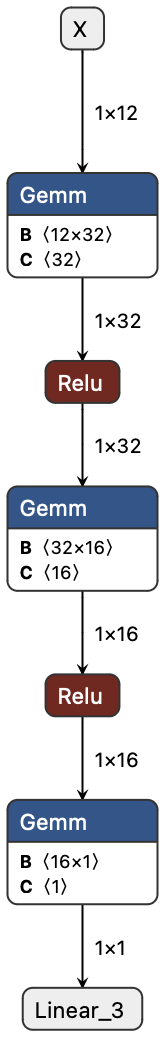
\includegraphics[scale=0.3]{"Chapter7/img/AC1.png"}
    \end{figure}

    \item \textbf{CARTPOLE network:}\\  
    \begin{figure}[]
        \caption{\label{fig:cartpole-network} Example of the structure of the cartpole network}
        \centering
        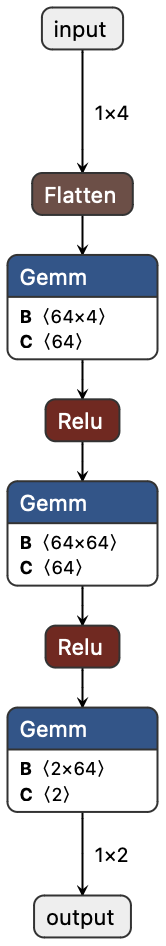
\includegraphics[scale=0.4]{"Chapter7/img/cartpole.png"}
    \end{figure}
    CARTPOLE is a classic control problem in the field of reinforcement learning, often used as a benchmark task. In CARTPOLE, the goal is to balance a pole on top of a cart that can move horizontally along a track. 
    The agent must apply appropriate actions to keep the pole upright for as long as possible.
    A neural network can be used as a function approximator to learn a policy for the CARTPOLE task. The neural network takes the current state of the cart and pole as input and outputs the action to be taken. 
    The state representation typically includes variables such as the cart's position, velocity, pole angle, and angular velocity.
    The network architecture consists of two fully connected layers of 64 hidden neurons, each followed by a ReLU acti- vation, and a last fully connected layer of 2 neurons without a following activation function. 
    The graphical representation of a neural network architecture of this kind is displayed in FIG~\ref{fig:cartpole-network}.

    \item \textbf{DUBINSREJOIN network:}
    \begin{figure}[H]
        \caption{\label{fig:dubins-network} Example of the structure of the dubinsrejoin network}
        \centering
        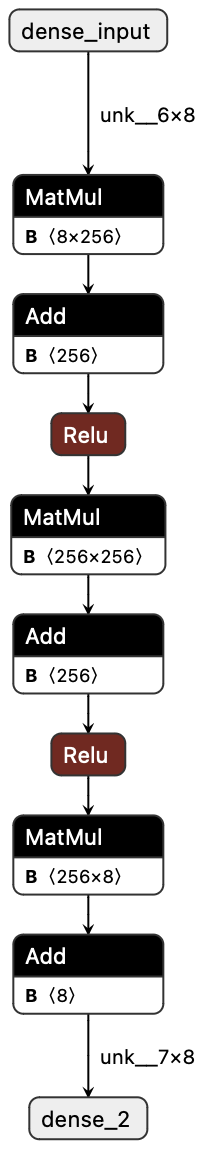
\includegraphics[scale=0.4]{"Chapter7/img/dubinsrejoin.png"}
    \end{figure}
    This case study focuses on training an unmanned aerial vehicle, called the wingman, to fly in formation with a manned vehicle known as the lead. The specific task addressed is the 2D version of this problem, where the reinforcement learning (RL) agent must learn how to control the wingman's position relative to the lead. The inputs to the RL agent are the position, heading, and velocity of both the lead and the wingman, while the outputs are a combination of eight real values representing various commands.
    The network architecture used in this case study consists of three fully connected layers, each containing 256 hidden neurons. ReLU activation functions are applied after the first two layers, except for the last layer.

    \item \textbf{LUNARLANDER network:}
    \begin{figure}[H]
        \caption{\label{fig:lunarlander-network} Example of the structure of the lunarlander network}
        \centering
        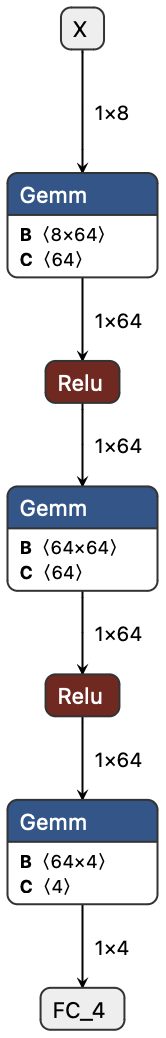
\includegraphics[scale=0.4]{"Chapter7/img/lunarlander.png"}
    \end{figure}
    This case study focuses on a rocket trajectory optimization problem, specifically landing a lander on a designated landing pad in a two-dimensional space. 
    The network has 8 real-value inputs, representing the coordinates, velocity, linear velocity, angle, angular velocity, and leg contact information of the lander. 
    The outputs consist of four real values, determining the lander's action: do nothing, fire left orientation engine, fire main engine, or fire right orientation engine. 
    The network architecture consists of three fully connected layers with 64 hidden neurons each, using ReLU activation except for the last layer.
    
\end{itemize}

\subsection{Validation test and results}
In this subsection, we present the tests conducted to verify the correct functioning of bound propagation.
In order to ensure the accuracy of the results, a second implementation of bound propagation was developed, which utilizes the linearization of the Rectified Linear Unit (ReLU) as depicted in subsection~\ref{subsec:symbolic-linear-relaxation}. 
This step was taken to validate the consistency of the results with the actual more complex and less intuitive linearization used in practice.
Subsequently, both implementations of bound propagation were applied to different neural networks, and a set of representative properties was selected for testing purposes. 
By subjecting these networks to the two bound propagation methods, we aimed to compare their results and evaluate their effectiveness in determining the lower and upper bounds of the network's output.
Moreover, to ensure the proper integration of the implemented algorithms with PyNeVer, an additional algorithm was developed. 
This algorithm was responsible for collecting the stars generated during the "complete" verification process and extracting the corresponding lower and upper bounds for each node in every layer of the neural network.
By conducting these tests and implementing the necessary procedures for interfacing with PyNeVer, we were able to validate the correct functioning of the bound propagation methods and obtain the desired bounds for further analysis and verification.\\

Thanks to the precise nature of PyNeVer's "complete" verification, we can accurately identify and quantify both stable and unstable nodes. In contrast, the bound propagation method only provides information about the stable nodes, leaving the true nature of classified unstable nodes uncertain. 
As bound propagation is an over-approximation technique, some nodes classified as unstable by bound propagation may actually be stable in reality.
In the graphs presented, we not only showcase the stable nodes but also highlight the number of nodes that are not captured due to the inherent over-approximation of bound propagation. These are nodes 
that are stable but wrongly classified as unstable by the bound propagation method. By quantifying this discrepancy, we gain insights into the potential room for improvement in bound propagation.
This analysis allows us to understand the limitations and possible inaccuracies associated with bound propagation, guiding us in exploring ways to enhance its performance. 
By comparing the results from bound propagation with the ground truth provided by PyNeVer's "complete" verification, we can measure the extent to which bound propagation aligns with the actual stability of nodes. 
This quantitative assessment provides valuable information about the reliability and potential areas for refinement in the bound propagation method.
The tests were conducted on a subset of networks or properties, specifically for ACAS, CARTPOLE, and ACC networks, which are relatively small. An attempt was made to perform a complete verification on the DUBINSREJOIN network, but due to its layer of 256 neurons, it required excessive time to complete the verification process.

% In this subsection, the method for checking the correctness and coherence of bound propagation results is described. The objective was to ensure that the utilized bound propagation method was effectively overestimating the true bounds. However, calculating the real bounds accurately was challenging due to the non-linearity of the ReLU activation function. 
% Fortunately, a complete verification method with exponential complexity was employed by collecting all the generated states during the algorithm, enabling the calculation of the real bounds.
% The tests were conducted on a subset of networks or properties, specifically for ACAS, CARTPOLE, and ACC networks, which are relatively small. An attempt was made to perform a complete verification on the DUBINSREJOIN network, but due to its layer of 256 neurons, it required excessive time to complete the verification process.
% To ensure the accuracy of the bounds, another version of bound propagation was implemented. This version utilized a different ReLU over-approximation technique. The purpose of this implementation was to verify that both bound propagation methods never underestimated the real bounds.
% Additionally, this approach allowed for counting the actual number of unstable nodes and comparing them with the number of unstable nodes classified by the two bound propagation methods used. 
% This comparison highlighted the differences in performance resulting from the choice of ReLU linearization technique
\begin{itemize}
    \item \textbf{ACAS Results:}\\
    In Table~\ref{table:ACAS-ANALISY}, nine different properties have been verified using PyNeVer and two different bound propagation BP1 and BP2 have been performed. The "NO BP" column displays the number of unstable nodes obtained. 
    The BP 1 columns displays the number of unstable nodes classified by BP 1, the same for BP 2.
    The "UNCATCHED NODES" refers to nodes that are classified as "unstable" due to the overapproximation introduced by ReLU linearization, but are actually stable. On average, we found 41.3 real unstable nodes. 
    However, "BP type 1" and "BP type 2" classify, on average, 84.6 and 101 nodes as "unstable," respectively. 5The results also show how the ReLU linearization used has on average better performance than the naive one used only for testing purposes.
    It is normal for Bound Propagation to introduce some errors. However, in the case of the ACAS network, we observed a higher number of "UNCATCHED NODES" compared to other networks analyzed. This is primarily due to the depth of the ACAS network. Deeper networks have more ReLU layers, which contribute to overapproximation and cause Bound Propagation to diverge faster.
   
    \begin{table}[H]
        \centering
        \resizebox{\columnwidth}{!}{%
        \begin{tabular}{@{}llllll@{}}
            \toprule
            \multicolumn{6}{c}{ACAS property: SMT3}  \\
            \cmidrule(r){1-6} 
            \multirow{2}{*}{NETWORK ID} &  \multicolumn{3}{c}{PYNEVER} &  \multicolumn{2}{c}{}\\ 
            \cmidrule(r){2-4}
                   & NO BP                                        & BP type 1                                     & BP type 2                                     & UNCATCHED NODES BP type 1               & UNCATCHED NODES BP type 2               \\\cmidrule(r){1-6}
        1\_1       & {\color[HTML]{D9E1F2} 58\textbackslash{}300} & {\color[HTML]{D9E1F2} 132\textbackslash{}300} & {\color[HTML]{D9E1F2} 148\textbackslash{}300} & {\color[HTML]{D9E1F2} 74}         & {\color[HTML]{D9E1F2} 90}         \\
        1\_3       & {\color[HTML]{D9E1F2} 43\textbackslash{}300} & {\color[HTML]{D9E1F2} 134\textbackslash{}300} & {\color[HTML]{D9E1F2} 152\textbackslash{}300} & {\color[HTML]{D9E1F2} 91}         & {\color[HTML]{D9E1F2} 109}        \\
        1\_4       & {\color[HTML]{D9E1F2} 28\textbackslash{}300} & {\color[HTML]{D9E1F2} 120\textbackslash{}300} & {\color[HTML]{D9E1F2} 137\textbackslash{}300} & {\color[HTML]{D9E1F2} 92}         & {\color[HTML]{D9E1F2} 109}        \\
        1\_5       & {\color[HTML]{D9E1F2} 27\textbackslash{}300} & {\color[HTML]{D9E1F2} 118\textbackslash{}300} & {\color[HTML]{D9E1F2} 145\textbackslash{}300} & {\color[HTML]{D9E1F2} 91}         & {\color[HTML]{D9E1F2} 118}        \\
        2\_3       & {\color[HTML]{D9E1F2} 42\textbackslash{}300} & {\color[HTML]{D9E1F2} 107\textbackslash{}300} & {\color[HTML]{D9E1F2} 108\textbackslash{}300} & {\color[HTML]{D9E1F2} 65}         & {\color[HTML]{D9E1F2} 66}         \\
        3\_2       & {\color[HTML]{D9E1F2} 39\textbackslash{}300} & {\color[HTML]{D9E1F2} 154\textbackslash{}300} & {\color[HTML]{D9E1F2} 177\textbackslash{}300} & {\color[HTML]{D9E1F2} 115}        & {\color[HTML]{D9E1F2} 138}        \\
        4\_2       & {\color[HTML]{D9E1F2} 49\textbackslash{}300} & {\color[HTML]{D9E1F2} 124\textbackslash{}300} & {\color[HTML]{D9E1F2} 138\textbackslash{}300} & {\color[HTML]{D9E1F2} 75}         & {\color[HTML]{D9E1F2} 89}         \\
        4\_3       & {\color[HTML]{D9E1F2} 42\textbackslash{}300} & {\color[HTML]{D9E1F2} 128\textbackslash{}300} & {\color[HTML]{D9E1F2} 138\textbackslash{}300} & {\color[HTML]{D9E1F2} 86}         & {\color[HTML]{D9E1F2} 96}         \\
        5\_1       & {\color[HTML]{D9E1F2} 44\textbackslash{}300} & {\color[HTML]{D9E1F2} 117\textbackslash{}300} & {\color[HTML]{D9E1F2} 138\textbackslash{}300} & {\color[HTML]{D9E1F2} 73}         & {\color[HTML]{D9E1F2} 94}         \\\cmidrule(r){1-6}
        average:   &  {\color[HTML]{FF0000}41.3\textbackslash{}300} &  {\color[HTML]{FF0000}126\textbackslash{}300} & {\color[HTML]{FF0000}142.3\textbackslash{}300}  & {\color[HTML]{FF0000} leaks: 762  average: 84.6} & {\color[HTML]{FF0000} leaks: 909  average: 101} \\\cmidrule(r){1-6}
        \end{tabular}%
        }
        \caption{This table shows the results got by tests performed on SMT3 property and some randomly chosen networks. The networs have all the same structure but different weight and bias fully connected matrices. In total the ACAS has 350 but we take account on only the first 300 because the last fc layer is excluded.}
        \label{table:ACAS-ANALISY}
    \end{table}

    
    \item \textbf{AC Results:} \\
    In Table~\ref{table:AC-ANALISY}, four different ACC networks have been verified with a randomly generated property. As mentioned earlier, two backpropagation (BP) algorithms, BP 1 and BP 2, were applied to these networks.
    Since we are comparing networks with different depths, calculating the average number of unstable nodes becomes meaningless. Therefore, it has not been included in the table.
    It's important to note that these networks have a lesser depth compared to ACAS networks. Consequently, the number of uncaptured nodes is relatively smaller. Interestingly, in this scenario, BP 2 performs better than BP 1.
    Overall, the table presents the results of the verification process for the ACC networks and their performance under the given property. The comparison between the two BP algorithms provides insights into their effectiveness in dealing with the specific networks and property involved.

    \begin{table}[H]
        \centering
        \resizebox{\columnwidth}{!}{%
        \begin{tabular}{@{}lllllll@{}}
            \toprule
            \multicolumn{6}{c}{ACC}  \\
            \cmidrule(r){1-6} 
            \multirow{2}{*}{NETWORK ID} &  \multicolumn{3}{c}{PYNEVER} &  \multicolumn{2}{c}{}\\ 
            \cmidrule(r){2-4}
                 & NO BP               & BP type 1                 & BP type 2 & UNCATCHED NODES BP type 1            & UNCATCHED NODES BP type 2            \\\cmidrule(r){1-6}
        1        & {\color[HTML]{ACB9CA} 23/48} & {\color[HTML]{ACB9CA} 25/48} & {\color[HTML]{ACB9CA} 23/48}        & {\color[HTML]{ACB9CA} 3}                              & {\color[HTML]{ACB9CA} 1}                              \\
        2        & {\color[HTML]{ACB9CA} 11/96} & {\color[HTML]{ACB9CA} 11/96} & {\color[HTML]{ACB9CA} 11/96}        & {\color[HTML]{ACB9CA} 0}                              & {\color[HTML]{ACB9CA} 0}                              \\
        5        & {\color[HTML]{ACB9CA} 16/56} & {\color[HTML]{ACB9CA} 18/56} & {\color[HTML]{ACB9CA} 18/56}        & {\color[HTML]{ACB9CA} 2}                              & {\color[HTML]{ACB9CA} 2}                              \\
        6        & {\color[HTML]{ACB9CA} 18/112}& {\color[HTML]{ACB9CA} 19/112}& {\color[HTML]{ACB9CA} 19/112}       & {\color[HTML]{ACB9CA} 1}                              & {\color[HTML]{ACB9CA} 1}                              \\\cmidrule(r){1-6}
                 &                              &                              &              & {\color[HTML]{FF0000} leak: 6} & {\color[HTML]{FF0000} leak: 4} \\\cmidrule(r){1-6}
    
        \end{tabular}%
        }
        \caption{This is the caption for the first table.}
        \label{table:AC-ANALISY}
        \caption{This table shows the results of AC networks on random generated properties. The structure of the different netowork is different. The netowork id is ascending sorted respect to the number of neurons. }
    \end{table}

    \item \textbf{CARTPOLE Results:}\\
    In Table~\ref{table:CARTPOLE-ANALISY}, ten different CARTPOLE properties have been verified. Due to the fact that CARTPOLE network is very small and shallow, the number of UNCATCHED NODES is 0.  

    \begin{table}[H]
        \centering
        \resizebox{\columnwidth}{!}{%
        \begin{tabular}{@{}llllll@{}}
            \toprule
            \multicolumn{6}{c}{CARTPOLE}  \\
            \cmidrule(r){1-6} 
            \multirow{2}{*}{PROPERTY ID} &  \multicolumn{3}{c}{PYNEVER} &  \multicolumn{2}{c}{}\\ 
            \cmidrule(r){2-4}
                    & NO BP & BP type 1 & BP type 2 & UNCATCHED NODES BP type 1            & UNCATCHED NODES BP type 2              \\\cmidrule(r){1-6}
        1           & 5             & 5            & 5            & 0                              & 0                              \\
        2           & 16            & 16           & 16           & 0                              & 0                              \\
        3           & 5             & 5            & 5            & 0                              & 0                              \\
        4           & 15            & 15           & 15           & 0                              & 0                              \\
        5           & 19            & 19           & 19           & 0                              & 0                              \\
        9           & 0             & 0            & 0            & 0                              & 0                              \\
        14          & 3             & 3            & 3            & 0                              & 0                              \\
        27          & 2             & 2            & 2            & 0                              & 0                              \\
        39          & 2             & 2            & 2            & 0                              & 0                              \\
        45          & 1             & 1            & 1            & 0                              & 0                              \\\cmidrule(r){1-6}
                    &               &              &              & {\color[HTML]{FF0000} leak: 0} & {\color[HTML]{FF0000} leak: 0} \\\cmidrule(r){1-6}
        \end{tabular}%
        }
        \label{table:CARTPOLE-ANALISY}
        \caption{This table shows the results of CARTPOLE netowrk tested with different properties.}
        \end{table}

    \item \textbf{DUBINSREJOIN Results:} \\
    Due to the size of the layers in the DuBINSREJOIN network, the first layer has 256 nodes, and verifying a property with such a large network exceeds the time limit set at 15 minutes as shown in Table~\ref{table:DUBINS}. 
    Therefore, the results shown in the table only display the number of unstable nodes for each layer obtained using Bound Propagation BP 1, and not those obtained by performing a post-analysis on the stars. 
    The test was conducted on only one property to provide an overestimated estimate of the number of stars and consequently explain why the verification process was so slow.

    \begin{table}[H]        
        \centering
        \begin{tabular}{lll}
        \toprule
        \multicolumn{3}{c}{DUBINS}  \\
        \cmidrule(r){1-3}
                        & FC1                                & FC2                                \\
        UNSTABLE NODES  & {\color[HTML]{B4C6E7} 106/256}     & {\color[HTML]{B4C6E7} 104/256}     \\
        NUMBER OF STARS & {\color[HTML]{C00000} 8.11296E+31} & {\color[HTML]{C00000} 2.02824E+31}
        \end{tabular}
        \label{table:DUBINS-ANALISY}
    \end{table}

    As shown in Table~\ref{table:DUBINS-ANALISY}, the number of stars blows up (exponential complexity). In total we have $2^{106}$ stars in input in the ReLU layer after the first fc layer and  at most $(2^{106})*(2^{104})$ stars in input to the second ReLU layer.

\end{itemize}

\subsection{Time/Memory usage test}
In this subsection, the data obtained from time and memory usage testing is presented. The tests were conducted on ACAS, AC, CARTPOLE, DUBINSREJOIN, and LUNARLANDER networks. In the first phase, time tests were performed to measure the time required by the networks to verify properties using both the original PyNeVer algorithm and the one with implemented Bound Propagation. The results were promising, as the performance of the algorithm with Bound Propagation showed improvements ranging from 10\% to 45\% compared to the original algorithm. 
The graphs indicate that networks like ACAS in Table~\ref{table:ACAS} and CARTPOLE in Table~\ref{table:CARTPOLE} had an average performance gain of 10\%, while networks like AC in Table~\ref{table:AC} and LUNARLANDER in Table~\ref{table:LUNAR} had an average performance gain of 45\%. These performance differences are influenced by factors such as network depth and layer size.
For example, networks with a few fully connected layers but many nodes showed performance gains because the large number of nodes increased the likelihood of having unstable nodes, resulting in more stars being generated. And the more stars we have the more GET\_BOUND operations are saved in case of a classified STABLE node. Additionally, the shallow depth of the network reduced the over-approximation introduced by bound propagation, resulting in fewer misclassified nodes (UNCATCHED NODES). This led to a reduction in the number of calls to the GET\_BOUNDS function and improved performance.
In the second part of the tests, the performance of the verification algorithm of the 2021 VNNCOMP winners, specifically ABCrown, was compared to the PyNeVer algorithm with Bound Propagation. Although the implemented Bound Propagation improved the performance and reduced the performance gap between PyNeVer and ABCrown, there is still an order of magnitude difference between the two algorithms in some networks like LUNARLANDER.
In the third phase, the peak RAM usage of both versions of PyNeVer was compared. The results in Table~\ref{table:memory-results} showed that the version with Bound Propagation had an increase of only 0-1\% in memory usage compared to the original version.\\
In order to measure the memory used during the verification process it has been imported the python library \textbf{tracemalloc}. 
The tracemalloc module is a debug tool to trace memory blocks allocated by Python. It provides the following information:

\begin{itemize}
\item Tracing the allocation: The module allows you to trace the traceback (call stack) where an object was allocated, helping to identify the source of memory allocations.
\item Statistics on allocated memory blocks: tracemalloc provides statistics on allocated memory blocks, categorized by filename and line number. These statistics include the total size of allocated memory blocks, the number of allocations per line, and the average size of allocated memory blocks.
\item Memory leak detection: By capturing two snapshots at different points in the program's execution, you can use tracemalloc to compute the differences between the snapshots and detect memory leaks, which occur when memory is allocated but not properly released.
\end{itemize}
In order to measure the memory peak during the verification process, get\_traced\_memory has bees used. This tracemalloc method gets the current size and peak size of memory blocks traced by the tracemalloc module as a tuple.\\

By leveraging the capabilities of the tracemalloc module, you can track and analyze the memory allocation patterns of your Python program, identify memory-intensive sections, and detect potential memory leaks.
Therefore, considering the significant improvement in terms of time and the negligible increase in RAM usage, it can be concluded that Bound Propagation has made the PyNeVer algorithm more efficient without any negative drawbacks.
These findings demonstrate the effectiveness of Bound Propagation in enhancing the performance of the PyNeVer algorithm, making it a valuable addition to the verification process for neural networks.

\begin{table}[]
    \resizebox{\columnwidth}{!}{%
    \begin{tabular}{@{}lllllll@{}}
    \toprule
    \multirow{2}{*}{Network id} & \multicolumn{2}{c}{PyNeVer with BP} & \multicolumn{2}{c}{PyNeVer without BP} \\ 
    \cmidrule(r){2-3}
    \cmidrule(r){4-5}
            & prop1                             & prop2                                         & prop1                             & prop2                                         & prop1 GAIN                        & prop2 GAIN                        \\ \cmidrule(r){1-7}
    AC1     & {\color[HTML]{ACB9CA} 0.96861878} & {\color[HTML]{ACB9CA} 8.51528863}             & {\color[HTML]{ACB9CA} 1.34609463} & {\color[HTML]{ACB9CA} 15.0083293}             & {\color[HTML]{ACB9CA} 0.28042296} & {\color[HTML]{ACB9CA} 0.43262914} \\
    AC2     & {\color[HTML]{ACB9CA} 0.89786378} & {\color[HTML]{ACB9CA} 28.2898089}             & {\color[HTML]{ACB9CA} 1.07707785} & {\color[HTML]{ACB9CA} 75.0877929}             & {\color[HTML]{ACB9CA} 0.16638915} & {\color[HTML]{ACB9CA} 0.62324357} \\
    AC3     & {\color[HTML]{ACB9CA} 1.32726333} & {\color[HTML]{ACB9CA} time\_limit\_exception} & {\color[HTML]{ACB9CA} 2.82069459} & {\color[HTML]{ACB9CA} time\_limit\_exception} & {\color[HTML]{ACB9CA} 0.52945514} & {\color[HTML]{ACB9CA} NAN}        \\ 
    AC4     & {\color[HTML]{ACB9CA} 22.1184216} & {\color[HTML]{ACB9CA} time\_limit\_exception} & {\color[HTML]{ACB9CA} 169.126968} & {\color[HTML]{ACB9CA} time\_limit\_exception} & {\color[HTML]{ACB9CA} 0.86922002} & {\color[HTML]{ACB9CA} NAN}        \\
    AC5     & {\color[HTML]{ACB9CA} 1.27058169} & {\color[HTML]{ACB9CA} 37.5357738}             & {\color[HTML]{ACB9CA} 1.34696131} & {\color[HTML]{ACB9CA} 43.3556351}             & {\color[HTML]{ACB9CA} 0.05670514} & {\color[HTML]{ACB9CA} 0.13423541} \\
    AC6     & {\color[HTML]{ACB9CA} 1.25507795} & {\color[HTML]{ACB9CA} 103.394566}             & {\color[HTML]{ACB9CA} 1.52465712} & {\color[HTML]{ACB9CA} 270.691961}             & {\color[HTML]{ACB9CA} 0.17681298} & {\color[HTML]{ACB9CA} 0.61803607} \\
    AC7     & {\color[HTML]{ACB9CA} 1.71481047} & {\color[HTML]{ACB9CA} time\_limit\_exception} & {\color[HTML]{ACB9CA} 3.01721494} & {\color[HTML]{ACB9CA} time\_limit\_exception} & {\color[HTML]{ACB9CA} 0.43165783} & {\color[HTML]{ACB9CA} NAN}        \\
    AC8     & {\color[HTML]{ACB9CA} 2.64424206} & {\color[HTML]{ACB9CA} time\_limit\_exception} & {\color[HTML]{ACB9CA} 8.24535111} & {\color[HTML]{ACB9CA} time\_limit\_exception} & {\color[HTML]{ACB9CA} 0.6793051}  & {\color[HTML]{ACB9CA} NAN}        \\ \cmidrule(r){1-7}
    PyNeVer relative improvement:        &                                   &                                               &                                   &                                               & {\color[HTML]{FF0000} 40\%}       & {\color[HTML]{FF0000} 45\%}       \\ \cmidrule(r){1-7}
    \end{tabular}%
    }
    \caption{This table shows the test results on AC network on two different properties.}
    \label{table:AC}
\end{table}


\begin{table}[]
    \centering
    \resizebox{\columnwidth}{!}{%
    \begin{tabular}{lllllll}
    \toprule
    \multirow{2}{*}{ACAS id} & \multicolumn{2}{c}{PyNeVer with BP} & \multicolumn{2}{c}{PyNeVer without BP} \\ 
    \cmidrule(r){2-3}
    \cmidrule(r){4-5}
                                & SMT3                              & SMT4                              & SMT3                              & SMT4                              & GAIN SMT3                   & GAIN SMT4                   \\\cmidrule(r){1-7}
    1\_1                        & {\color[HTML]{ACB9CA} 81.6150596} & {\color[HTML]{ACB9CA} 33.6213214} & {\color[HTML]{ACB9CA} 84.8323429} & {\color[HTML]{ACB9CA} 35.5213297} & {\color[HTML]{ACB9CA} 3.22} & {\color[HTML]{ACB9CA} 1.90} \\
    1\_2                        & {\color[HTML]{ACB9CA} 50.0253018} & {\color[HTML]{ACB9CA} 21.7184501} & {\color[HTML]{ACB9CA} 57.3484051} & {\color[HTML]{ACB9CA} 24.2984346} & {\color[HTML]{ACB9CA} 7.32} & {\color[HTML]{ACB9CA} 2.58} \\
    2\_1                        & {\color[HTML]{ACB9CA} 19.6118035} & {\color[HTML]{ACB9CA} 12.0285352} & {\color[HTML]{ACB9CA} 21.1221661} & {\color[HTML]{ACB9CA} 14.7471417} & {\color[HTML]{ACB9CA} 1.51} & {\color[HTML]{ACB9CA} 2.72} \\
    2\_2                        & {\color[HTML]{ACB9CA} 13.0979525} & {\color[HTML]{ACB9CA} 9.96734113} & {\color[HTML]{ACB9CA} 14.3491091} & {\color[HTML]{ACB9CA} 11.0515448} & {\color[HTML]{ACB9CA} 1.25} & {\color[HTML]{ACB9CA} 1.08} \\
    3\_1                        & {\color[HTML]{ACB9CA} 12.3011813} & {\color[HTML]{ACB9CA} 19.6764414} & {\color[HTML]{ACB9CA} 13.9424404} & {\color[HTML]{ACB9CA} 20.9019084} & {\color[HTML]{ACB9CA} 1.64} & {\color[HTML]{ACB9CA} 1.23} \\
    3\_2                        & {\color[HTML]{ACB9CA} 77.6160142} & {\color[HTML]{ACB9CA} 14.2753579} & {\color[HTML]{ACB9CA} 85.8698075} & {\color[HTML]{ACB9CA} 16.3781728} & {\color[HTML]{ACB9CA} 8.25} & {\color[HTML]{ACB9CA} 2.10} \\
    4\_1                        & {\color[HTML]{ACB9CA} 5.62614266} & {\color[HTML]{ACB9CA} 5.36426193} & {\color[HTML]{ACB9CA} 6.14406902} & {\color[HTML]{ACB9CA} 5.91605551} & {\color[HTML]{ACB9CA} 0.52} & {\color[HTML]{ACB9CA} 0.55} \\
    4\_2                        & {\color[HTML]{ACB9CA} 11.8124654} & {\color[HTML]{ACB9CA} 33.7138488} & {\color[HTML]{ACB9CA} 13.1458899} & {\color[HTML]{ACB9CA} 36.6005748} & {\color[HTML]{ACB9CA} 1.33} & {\color[HTML]{ACB9CA} 2.89} \\
    5\_1                        & {\color[HTML]{ACB9CA} 10.3131805} & {\color[HTML]{ACB9CA} 5.42253668} & {\color[HTML]{ACB9CA} 11.8937659} & {\color[HTML]{ACB9CA} 5.9943051}  & {\color[HTML]{ACB9CA} 1.58} & {\color[HTML]{ACB9CA} 0.57} \\
    5\_2                        & {\color[HTML]{ACB9CA} 4.26043663} & {\color[HTML]{ACB9CA} 12.6508114} & {\color[HTML]{ACB9CA} 5.00902677} & {\color[HTML]{ACB9CA} 13.8963645} & {\color[HTML]{ACB9CA} 0.75} & {\color[HTML]{ACB9CA} 1.25} \\\cmidrule(r){1-7}
                                &                                   &                                   &                                   &                                   & {\color[HTML]{FF0000} 10\%} & {\color[HTML]{FF0000} 10\%} \\\cmidrule(r){1-7}      
    \end{tabular}%
    }
    \caption{This table shows the test results on ACAS network on two different properties.}
    \label{table:ACAS}
    \end{table}


\begin{table}[]
    \centering
    \begin{tabular}{@{}llll@{}}
    \toprule
    property\_id & PyNeVer with BP                               & PyNeVer without BP                            &  \\ \cmidrule(r){1-3}
    3            & {\color[HTML]{ACB9CA} time\_limit\_exception} & {\color[HTML]{ACB9CA} time\_limit\_exception} &  \\
    6            & {\color[HTML]{ACB9CA} time\_limit\_exception} & {\color[HTML]{ACB9CA} time\_limit\_exception} &  \\
    12           & {\color[HTML]{ACB9CA} time\_limit\_exception} & {\color[HTML]{ACB9CA} time\_limit\_exception} &  \\ \cmidrule(r){1-3}
    \end{tabular}%
    \caption{This table shows the test results on DUBINSREJOIN network on three different properties.}
    \label{table:DUBINS}
\end{table}


\begin{table}[]
    \centering
    \begin{tabular}{@{}llll@{}}
        \toprule
        \multicolumn{4}{c}{Cartpole}  \\
        \cmidrule(r){1-4}
                                            & PyNeVer with BP                        & PyNeVer without BP               & ABCROWN                           \\ \cmidrule(r){1-4}
    time(s):                                & {\color[HTML]{ACB9CA} 0.93486845}      & {\color[HTML]{ACB9CA} 0.815644} & {\color[HTML]{ACB9CA} 0.20461254}  \\ \cmidrule(r){1-4}
    PyNeVer relative improvement:           &                                        & {\color[HTML]{FF0000} 8\%}       &                                   \\ \cmidrule(r){1-4}
    \end{tabular}
    \caption{This table shows the test results on CARTPOLE network on two different properties.}
    \label{table:CARTPOLE}
\end{table}


\begin{table}[]
    \centering
    \begin{tabular}{@{}llll@{}}
        \toprule
        \multicolumn{4}{c}{Lunar}  \\
        \cmidrule(r){1-4}
                                             & PyNeVer with BP & PyNeVer without BP                & ABCROWN                           \\ \cmidrule(r){1-4}
    time(s):                                 & {\color[HTML]{ACB9CA} 7.34236826922983}                   & {\color[HTML]{ACB9CA} 13.7997844442866}  & {\color[HTML]{ACB9CA} 0.10526261230699} \\ \cmidrule(r){1-4}
    PyNeVer relative improvement:            &                                                     & {\color[HTML]{FF0000} 45\%}       &                                   \\ \cmidrule(r){1-4}
    \end{tabular}
    \caption{This is the caption for the first table.}
    \label{table:LUNAR}
\end{table}


    \begin{table}[htbp]
        \begin{minipage}{0.45\linewidth}
        \centering
        \begin{tabular}{@{}ll@{}}
        \toprule
        \multicolumn{2}{c}{AC}  \\\cmidrule{1-2}
        NO BP                                & BP type 1                         \\\cmidrule{1-2}
        {\color[HTML]{D9E1F2} 55.9687 MB} & {\color[HTML]{D9E1F2} 56.02 MB} \\\cmidrule{1-2}
        \end{tabular}      
        %\caption{Tabella 1}
        \end{minipage}\hfill
        \begin{minipage}{0.45\linewidth}
        \centering
        \begin{tabular}{@{}ll@{}}
        \toprule
        \multicolumn{2}{c}{ACAS}  \\\cmidrule{1-2}
        NO BP                              & BP type 1                           \\\cmidrule{1-2}
        {\color[HTML]{D9E1F2} 48.8035 MB} & {\color[HTML]{D9E1F2} 50.6578 MB} \\\cmidrule{1-2}
        \end{tabular}
        %\caption{Tabella 2}
        \end{minipage}  
        \vspace{0.5cm} % Spazio verticale tra le tabelle 
        \begin{minipage}{0.45\linewidth}
        \centering
        \begin{tabular}{@{}ll@{}}
        \toprule
        \multicolumn{2}{c}{CARTPOLE}  \\\cmidrule{1-2}
        NO OP                            & BP type 1                    \\\cmidrule{1-2}
        {\color[HTML]{D9E1F2} 0.3483 MB} & {\color[HTML]{D9E1F2} 0.3957 MB} \\\cmidrule{1-2}
        \end{tabular}
        %\caption{Tabella 3}
        \end{minipage}\hfill
        \begin{minipage}{0.45\linewidth}
        \centering
        \begin{tabular}{@{}ll@{}}
        \toprule
        \multicolumn{2}{c}{LUNAR}  \\\cmidrule{1-2}
        NO BP                             & BP type 1                        \\\cmidrule{1-2}
        {\color[HTML]{D9E1F2} 35.0736 MB} & {\color[HTML]{D9E1F2} 34.9736 MB} \\\cmidrule{1-2}
        \end{tabular}
        %\caption{Tabella 4}
        \end{minipage}
        \caption{Memory peak esperiment results}
        \label{table:memory-results}
        \end{table}

\subsection{Problems found}
During the tests performed to verify the correctness of the results, a part of the code checked whether the lower and upper bounds of BP1 and BP2 were an overestimation or equal of the actual bounds calculated with PyNeVer. If this was not the case, violations were written to a file. The presence of violations was intended to reveal any logical errors in the implemented BPs.
It was found that there was a high number of violations in the bounds calculated by concretizing the ReLU layers, particularly for values near zero. Further investigation revealed a problem of \textbf{numerical instability}, where PyNeVer expressed values that should be zero as extremely small negative numbers ($<10^{17}$).
It occurs when the numerical methods or algorithms used to perform calculations are sensitive to these small perturbations, amplifying their effects and producing incorrect or unreliable results.
There are various factors that can contribute to numerical instability, such as the presence of round-off errors due to limited precision in numerical representations or the accumulation of errors through iterative calculations.
In the context of the described issue with PyNeVer, the numerical instability led to small negative values being computed instead of zeros as in red in Table~\ref{table:violations}, potentially affecting the accuracy of the bounds calculated for ReLU layers. Identifying and addressing numerical instability is important to ensure the reliability and accuracy of numerical computations in scientific and computational applications.
Fortunately, these issues of numerical instability do not affect the functionality of PyNeVer in normal usage conditions, as they were observed only in the calculation of bounds for ReLU layer nodes, which was specifically forced for testing purposes. However, it was valuable to identify this type of problem in order to improve this aspect of the software in the future.

% Please add the following required packages to your document preamble:
% \usepackage[table,xcdraw]{xcolor}
% If you use beamer only pass "xcolor=table" option, i.e. \documentclass[xcolor=table]{beamer}
% \usepackage{longtable}
% Note: It may be necessary to compile the document several times to get a multi-page table to line up properly
% Please add the following required packages to your document preamble:
% \usepackage[table,xcdraw]{xcolor}
% If you use beamer only pass "xcolor=table" option, i.e. \documentclass[xcolor=table]{beamer}
% \usepackage{longtable}
% Note: It may be necessary to compile the document several times to get a multi-page table to line up properly
\
% Note: It may be necessary to compile the document several times to get a multi-page table to line up properly

\begin{longtable}{llll}
    \caption{This table shows the lower and upper bound of the first 2 layers, respectively a FC layer and a ReLU layer, of the ACAS\_1\_1 netowrk. In red are marked }
    \label{table:violations}\\
    \rowcolor[HTML]{92D050} 
    ABST\_FC\_0\_lower                 & ABST\_FC\_0\_upper                 & ABST\_ReLU\_0\_lower                                        & ABST\_ReLU\_0\_upper \\
    \endfirsthead
    %
    \endhead
    %
    {\color[HTML]{D9E1F2} 2.11417E-01} & {\color[HTML]{D9E1F2} 3.15850E-01} & 2.11417E-01                                                 & 3.15850E-01          \\
    4.93699E-02                        & 7.75720E-02                        & 4.93699E-02                                                 & 7.75720E-02          \\
    1.10239E-01                        & 2.20310E-01                        & 1.10239E-01                                                 & 2.20310E-01          \\
    1.05332E-01                        & 1.16736E-01                        & 1.05332E-01                                                 & 1.16736E-01          \\
    1.15834E-01                        & 1.72269E-01                        & 1.15834E-01                                                 & 1.72269E-01          \\
    -1.29774E+00                       & -1.24566E+00                       & 0.00000E+00                                                 & 0.00000E+00          \\
    -7.73407E-02                       & -3.26246E-02                       & 0.00000E+00                                                 & 0.00000E+00          \\
    5.47044E-02                        & 7.50849E-02                        & 5.47044E-02                                                 & 7.50849E-02          \\
    -2.64583E-02                       & 3.38720E-02                        & \cellcolor[HTML]{FFC7CE}{\color[HTML]{9C0006} -5.55112E-17} & 3.38720E-02          \\
    1.65018E-01                        & 1.73088E-01                        & 1.65018E-01                                                 & 1.73088E-01          \\
    -1.42997E-01                       & -9.35480E-02                       & 0.00000E+00                                                 & 0.00000E+00          \\
    -9.00223E-02                       & -7.31408E-02                       & 0.00000E+00                                                 & 0.00000E+00          \\
    2.38618E-01                        & 2.81425E-01                        & 2.38618E-01                                                 & 2.81425E-01          \\
    -4.20009E-01                       & -3.17158E-01                       & 0.00000E+00                                                 & 0.00000E+00          \\
    -1.83762E-01                       & -1.27231E-01                       & 0.00000E+00                                                 & 0.00000E+00          \\
    2.67941E-01                        & 3.27541E-01                        & 2.67941E-01                                                 & 3.27541E-01          \\
    -4.62791E-01                       & -3.69167E-01                       & 0.00000E+00                                                 & 0.00000E+00          \\
    -1.23659E+00                       & -1.20789E+00                       & 0.00000E+00                                                 & 0.00000E+00          \\
    -6.72436E-01                       & -6.35428E-01                       & 0.00000E+00                                                 & 0.00000E+00          \\
    -1.26407E-01                       & -1.05600E-01                       & 0.00000E+00                                                 & 0.00000E+00          \\
    1.23793E+00                        & 1.26081E+00                        & 1.23793E+00                                                 & 1.26081E+00          \\
    -8.50009E-01                       & -6.91952E-01                       & 0.00000E+00                                                 & 0.00000E+00          \\
    1.41420E-01                        & 2.34711E-01                        & 1.41420E-01                                                 & 2.34711E-01          \\
    1.83898E-01                        & 2.54354E-01                        & 1.83898E-01                                                 & 2.54354E-01          \\
    -2.12615E-02                       & -2.02086E-02                       & 0.00000E+00                                                 & 0.00000E+00          \\
    1.14649E-01                        & 1.34833E-01                        & 1.14649E-01                                                 & 1.34833E-01          \\
    1.78584E-02                        & 6.93870E-02                        & 1.78584E-02                                                 & 6.93870E-02          \\
    5.24102E-02                        & 1.29719E-01                        & 5.24102E-02                                                 & 1.29719E-01          \\
    -3.35602E-02                       & 1.80817E-02                        & \cellcolor[HTML]{FFC7CE}{\color[HTML]{9C0006} -5.55112E-17} & 1.80817E-02          \\
    -1.10612E+00                       & -9.19610E-01                       & 0.00000E+00                                                 & 0.00000E+00          \\
    5.97536E-02                        & 8.67993E-02                        & 5.97536E-02                                                 & 8.67993E-02          \\
    -1.61922E-01                       & -3.09046E-02                       & 0.00000E+00                                                 & 0.00000E+00          \\
    9.53638E-02                        & 1.13829E-01                        & 9.53638E-02                                                 & 1.13829E-01          \\
    3.38057E-02                        & 4.48437E-02                        & 3.38057E-02                                                 & 4.48437E-02          \\
    5.81427E-01                        & 6.27438E-01                        & 5.81427E-01                                                 & 6.27438E-01          \\
    -3.65423E-02                       & -5.21452E-03                       & 0.00000E+00                                                 & 0.00000E+00          \\
    1.62059E-01                        & 2.38890E-01                        & 1.62059E-01                                                 & 2.38890E-01          \\
    -2.78937E-02                       & 1.57217E-02                        & \cellcolor[HTML]{FFC7CE}{\color[HTML]{9C0006} -1.11022E-16} & 1.57217E-02          \\
    3.09683E-02                        & 4.27893E-02                        & 3.09683E-02                                                 & 4.27893E-02          \\
    -3.60360E-01                       & -1.88336E-01                       & 0.00000E+00                                                 & 0.00000E+00          \\
    3.03709E-01                        & 3.93415E-01                        & 3.03709E-01                                                 & 3.93415E-01          \\
    -4.37322E-01                       & -3.38209E-01                       & 0.00000E+00                                                 & 0.00000E+00          \\
    -1.27144E+00                       & -1.20366E+00                       & 0.00000E+00                                                 & 0.00000E+00          \\
    -2.66882E-02                       & -1.84704E-02                       & 0.00000E+00                                                 & 0.00000E+00          \\
    -5.29617E-02                       & 3.21762E-02                        & \cellcolor[HTML]{FFC7CE}{\color[HTML]{9C0006} -2.77556E-17} & 3.21762E-02          \\
    1.34893E-01                        & 1.55827E-01                        & 1.34893E-01                                                 & 1.55827E-01          \\
    2.31401E-02                        & 5.05105E-02                        & 2.31401E-02                                                 & 5.05105E-02          \\
    -2.89316E-01                       & -2.71779E-01                       & 0.00000E+00                                                 & 0.00000E+00          \\
    -2.90772E-02                       & -2.47172E-03                       & 0.00000E+00                                                 & 0.00000E+00          \\
    -2.76138E-02                       & 3.81140E-02                        & \cellcolor[HTML]{FFC7CE}{\color[HTML]{9C0006} -5.55112E-17} & 3.81140E-02         \\
    
    \end{longtable}
